Táto kapitola poslúži na opis niektorých problémov s ktorými sme sa stretli pri implementácii, popíše niektoré detialy implementácie a tiež aj rozdiely mezdi návrhom aplikácie a reálnou implementáciou aplikácie.
\section{Reprezentovanie herného sveta}
Keďže na implementáciu používame jazyk Java, tak sme sa na reprezentáciu herného sveta rozhodli použiť už implementovaný objekt v Jave. Využili sme na to, objekt HashMap, ktorý obsahuje zoznam kľúčov, na ktoré mapuje zadefinované objekty. My sme sa rozhodli klúče reprezentovať typom String a hodnoty, ktoré sú namapované na tieto Stringy sú typu Object.\par
Touto HashMapou simulujeme správanie predikátu. Vieme z nej dostať hodnotu podobne ako z predikátu, napríklad vieme si vypýtať namapovanú hodnotu na String ''princeplace'', čo nám povie kde sa princ v hernom svete nachádza. Takisto vieme zistiť hodnotu namapovanú na String ''fromcastleto'', ktorou je pole hodnôt, ktoré reprezentujú miesta do ktorých sa vieme presunúť z lokácie castle. Čiže napriíklad môžeme dostať hodnoty swamp,garden, jail a z tohto potom vieme povedať, že z lokácie castle sa môžeme presunúť do močiara, záhrady alebo väznice.\par
Mapovným typom je Object z dôvodu univerzálnosti hodnôt, ktoré naše simulované predikáty môžu poskytovať. Typ Object dedí v Jave každá trieda a teda hodnotou nášho simulovaného predikátu môže byť hocičo. Na našich príkladoch môžme vidieť využitie tohto faktu, jeden klúč vracia hodnotu String a druhý pole Stringov. Toto nám umožnuje mať jeden jediný objekt na popísanie celého herného sveta.
\subsection{Reprezentácia v súbore}
S reprezentáciou herného sveta súvisí aj jej zápis do súboru. Keďže máme svet reprezentovaný ako jediný objekt, tak sme sa rozhodli využiť knižnicu na skonvertovanie Javovského objektu do textového súboru.\par
Knižnicu, ktorú sme použili, je od spoločnosti Google a nazýva sa Gson. Táto knižnica umožňuje konvertovať objekty z Javy do textového súboru vo formáte JSON. JSON formát je celkom rozšíreným textovým formátom a teda jedna z výhod je aj že sú ľudia naň zvyknutý. Ak použijeme mód pekného vypisovania, tak je tento formát relatívne jednoduchý na čitanie pre človeka, tak ako sa požadovalo v návrhu. Na obrázku 4.1 môžeme vidieť čitateľnosť tohto formátu v móde pekného vypisovania.
\begin{figure}[H] 
\begin{center}
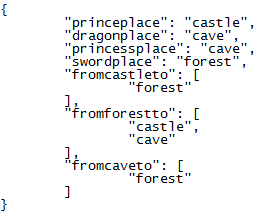
\includegraphics[scale=1.1]{img/subor_impl.png}
\caption{Ukážka formátu zápisu reprezentácie herného sveta do súboru.}
\label{fig:ch41}
\end{center}
\end{figure}
Ďaľšou výhodou je, že sme nemuseli implementovať vlastný parser pre načítavanie zo súboru, pretože knižnica obsahuje aj spätnú konverziu, teda zo súboru vo formáte JSON do daného objektu v Jave.\par
Jedinou nevýhodou je nemožnosť načítania objektu zo súboru ak je súbor v móde pekného vypisovania. Na načítanie objektu zo súboru musí byť súbor zapísaný v kompaktnom móde, čo znamená, že údaje sú zapísané v jednom riadku. Túto prekážku sme prekonali tak, že súbor v kompaktnom móde generujeme vždy a používateľovi poskytujeme pri zápise do súboru výber, či chce vygenerovať aj súbor v móde pekného vypisovania. Takto si používateľ vie vybrať, či bude chcieť daný súbor aj čítať a teda si vie vygenerovať aj pekne vypísaný súbor. Na druhú stranu ak používateľ reprezentáciu nebude chcieť čítať vlastnými očami tak mu nezahltíme systém zbytočnými súbormi. Použitie tejto knižnice je pre nás oveľa jednoduchšie ako implementovanie vlastného zapisovania do súboru a následného parsovania súboru pri načítavaní herného sveta zo súboru.
\section{Generovanie herného sveta}
Jednou z našich vymyslených zápletiek, je premôcť príšeru v hernom svete, ktorá blokuje jedu z ciest, ktrou sa váš hrdina môže vydať. Keď dané monštrum používateľ premôže tak sa mu uvoľní cesta, ktorú príšera blokovala. Táto udalosť je podľa nás zaujímavejšia ako väčšina ostatných akcií, ktoré hrdina môže vykonať a teda sme ju pre účely vyhľadávania ohodnotili nízkou cenou. A keďže naše plánovanie v podstate hľadá najzaujímavejší príbeh, lebo hľadá plán z najnižšou cenou, tak mohla nastať situácia, že plánovač našiel príbeh, ktorý zahŕňa aj boj s nejakým monštrom ale existovala aj nejaká dlhšia cesta k cieľu bez tejto udalosti a teda hráč mohol obísť našu vymyslenú zápletku a mohlo by sa mu zdať že daný vygenerovaný príbeh je mdlý. Kvôli tomuto fenoménu sme sa rozhodli trochu upraviť generovanie herného sveta.\par
Toto generovanie si zachováva vlastnosť náhodnosti, len je upravené tak aby bolo zaručené, že hráč bude musieť niekoľko krát bojovať s nejakým monštrom v rámci jedného príbehu. Generovanie sme upravili tak, že načítané lokácie rozdelíme do skupín. Medzi lokáciami v rámci jednej skupiny vygenerujeme náhodne hodnoty odkiaľ kam sa vieme presunúť a následne skupiny prepojíme príšerou, ktorá sa nachádza na jednej z lokácii v prvej skupine a blokuje cestu do niektorej lokácie z druhej skupiny. Týmto spôsobom vieme zreťaziť ľubovolný počet skupín. Na priblíženie tohto spôsobu generovania sveta použijeme konkrétny príklad znázornený aj na obrázku 4.2.
\begin{figure}[H] 
\begin{center}
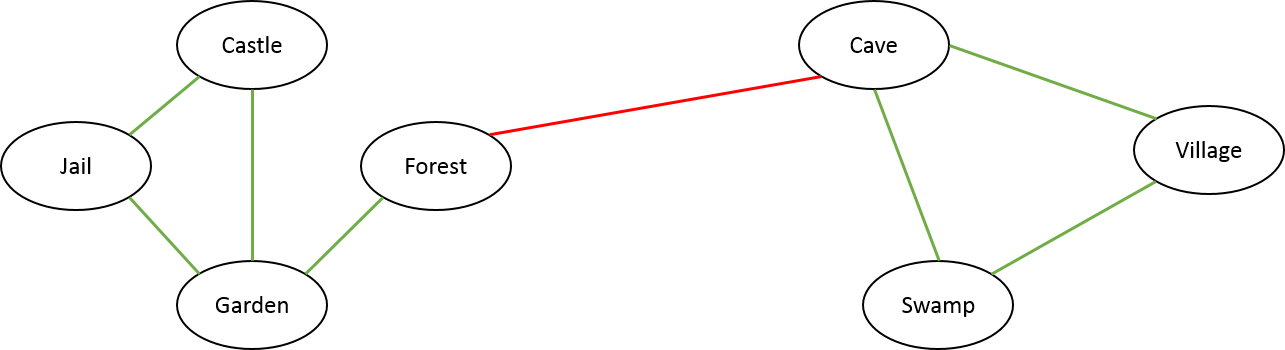
\includegraphics[scale=0.4]{img/gen_graf.png}
\caption{Grafická reprezentácia vygenerovaného herného sveta.}
\label{fig:ch42}
\end{center}
\end{figure}
V tomto prípade sme načítali sedem lokácii zo súboru, ktoré to sú vidieť na obrázku 4.2 reprezentované ako elipsy. Následne sme si lokácie rozdelili na dve skupiny v tomto prípade ľavú a pravú. V každej skupine zvlášť sme si vygenerovali cesty, tieto sú označené zelenou farbou. Potom sme vygenerovali náhodnú pozíciu príšery z ľavej skupiny lokácii, v tomto prípade je to Forest a zároveň sme vygenerovali náhodnú lokáciu, ktorú príšera blokuje z pravej skupiny, tou je miesto Cave. Teda vytvorili sme cestu z ľavej skupiny lokácii do pravej pomocou monštra, ktoré musí byť najprv porazené aby sa ňou dalo prejsť. Táto cesta je na obrázku 4.2 znázornená červenou farbou\par
V takto vygenerovanom svete, keď umiestnime cieľ hry do poslednej skupiny lokácii, tak máme zaručené, že ak náš plánovač nájde plán v ktorom sa nachádza akcia na boj s príšerou, tak sa pri hraní tohto sveta nedá táto akcia nijako obísť.
\section{Akcie a ich generovanie}
Akcie reprezentujeme podľa návrhu ako samostatné triedy. Jedna zmena oproti návrhu však nastala a to tá, že sme tieto triedy akcii vložili do samostatného Java balíčka, aby bola aplikácia prehľadnejšia.\par
Pri generovaní akcií sme chceli čo najviac zefektívniť plánovanie a teda pri generovaní herného sveta zisťujeme, ktoré objekty sa v ňom budú nachádzať a ktoré nie. Túto informáciu potom použijeme pri generovaní akcii aby sme limitovali počet akcií pre objekty, ktoré sa v hernom svete nenachádzajú. Čiže ak z piatich načítaných príšer pri generovaní herného sveta použijeme iba dve tak pri generovaní akcii vygenerujeme akcie len tým dvom príšerám, ktoré sa vo svete nachádzajú.\par
Ďaľšou takouto optimalizáciou je posienanie iba tých akcií, ktoré sa týkajú hrdinu príbehu. Keďže hrdina je hlavným poháňačom deja a tiež používateľ ovláda len tohto hrdinu, tak dáva zmyslel plánovať len tieto akcie.\par
Tieto dve optimalizácie znížia počet akcií používaných pri plánovaní, čo rapídne zníži počet potencionálnych stavov, ktoré treba prejsť pri plánovaní príbehu.
\section{Plánovací algoritmus}
Pri implementácii sme sa stretli s jedným závažným problémom a to, že náš plánovací algoritmus bol príliš neefektívny. Prehľadávať všetky možné cesty v grafe je zbytočné a časovo veľmi náročné. Rozhodli sme sa teda použiť ako plánovací algoritmus vyľadávanie A*, ktoré hľadá najkratšiu cestu v grafe. Tento prístup bol v podobnom kontexte využitý v článku\cite{astar}. Toto si nevyžadovalo veľké zmeny, keďže tento algoritmus sa vykonáva taktiež na grafoch. Zmeny, ktoré sme vykonali si popíšeme v tejto časti.\par
Jedným z aspektov, ktoré si vyhľadávanie A* vyžaduje je akási heuristika alebo niečo čo nám v priebehu vyhľadávania povie ako ďaľeko sme od cieľa. V našom prípade sme si vytvorili čiastkové cieľe príbehu a počet doteraz nevyriešených cieľov v aktuálnom stave sme použili ako túto heuristiku.\par
A* vyhľadávanie využíva prioritnú frontu na výber ďaľšieho vrcholu na spracovávanie. Aby sme mohli vytvoriť v Jave prioritnú frontu s triedou Node, čo je naša reprezentácia vrcholu, tak táto trieda musí implementovať funkciu compareTo(), ktorá sa používa na utriedenie fronty podľa priority. Túto funkciu sme implementovali tak, že spočítava zaujímavostnú hodnotu vrchola a počet nevyriešených čiastových cieľov v danom vrchole. Prioritná fronta sa usporadúva podľa tejto hodnoty vzostupne, aby sme vyberali stavy najbližšie k cieľu ako prvé.\par
Keď toto prehľadávanie nájde cestu do cieľového stavu, tak máme zaručené že sme našli najzaujímavejší príbeh daného sveta, pretože tento algoritmus hľadá najlacnejšiu cestu v grafe. Podobne ako v pôvodnom algoritme využijeme vrchol, ktorý reprezentuje cieľový stav na zrekonštruovanie celého nájdeného príbehu.\par
Táto zmena nám umožnila generovať oveľa dlhšie príbehy a za zlomok času oproti pôvodnému algoritmu.
\section{Ovládanie a hra}
Tak ako popisuje návrh ovládanie aplikácie je implementované cez konzolu. Používateľovi sa vypíšu do konzoli možnosti, ako je ukázané na obrázku 4.3, ktoré môže v danej chvíli vykonať. Tieto možnosti sú očíslované a používateľ zadaním príslušného čísla spustí daný príkaz.
\begin{figure}[H] 
\begin{center}
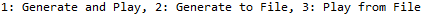
\includegraphics[scale=1.2]{img/menu.png}
\caption{Základné príkazy aplikácie.}
\label{fig:ch43}
\end{center}
\end{figure}
Po týchto prvých príkazoch, prichádza špecifikovanie vykonania vybraného príkazu. Napríklad pri vybraní prvého príkazu z obrázku 4.3 aplikácia potrebuje vedieť, či chceme hrať náhodný svet alebo svet vygenerovaný podľa nejakého semiačka, ako je zobrazené na obrázku 4.4.
\begin{figure}[H] 
\begin{center}
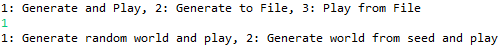
\includegraphics[scale=1.2]{img/menu2.png}
\caption{Špecifikujúce príkazy aplikácie.}
\label{fig:ch44}
\end{center}
\end{figure}
Niektoré z týchto špecifikačných príkazov zahŕňajú aj zadávanie rôznych vstupov používateľom. Ak si vyberieme v aplikácii generovanie herného sveta do súboru, tak tak aplikácia očakáva od používateľa boolovskú hodnotu, teda true alebo false, či chce vygenerovať aj súbor v móde pekného vypisovania (obr 4.5). Podobne pri náhodnom generovaní herného sveta do súboru si aplikácia vyžiada od používateľa aj počet svetov, ktoré chce používateľ vygenerovať (obr. 4.6).
\begin{figure}[H] 
\begin{center}
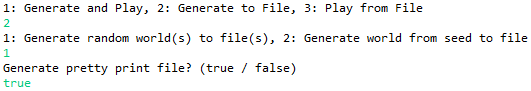
\includegraphics[scale=1.2]{img/menu3.png}
\caption{Zadávanie boolovských vstupov do aplikácie.}
\label{fig:ch45}
\end{center}
\end{figure}
\begin{figure}[H] 
\begin{center}
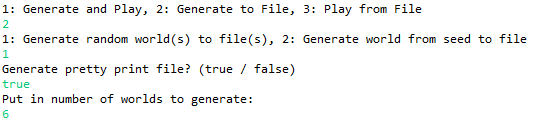
\includegraphics[scale=1.2]{img/menu4.png}
\caption{Zadávanie čisených vstupov do aplikácie.}
\label{fig:ch46}
\end{center}
\end{figure}
V prípade, keď generujeme herný svet zo súboru, tak sa od používateľa očakáva textový vstup, ktorým popíše relatívnu cestu ku textovému súboru formátu JSON, ktorý sa použije na generovanie herného sveta (obr. 4.7).
\begin{figure}[H] 
\begin{center}
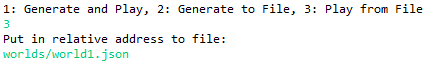
\includegraphics[scale=1.2]{img/menu5.png}
\caption{Zadávanie textových vstupov do aplikácie.}
\label{fig:ch47}
\end{center}
\end{figure}
Čo sa týka samotnej hry, tak každý herný ťah je opísaný pár riadkami, ako môžme vidieť na obrázku 4.8.
\begin{figure}[H] 
\begin{center}
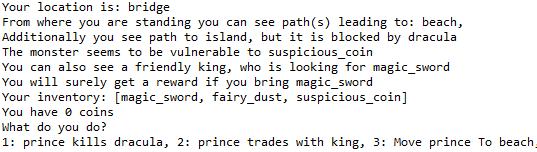
\includegraphics[scale=1.2]{img/turn.png}
\caption{Opis ťahu v aplikácii.}
\label{fig:ch48}
\end{center}
\end{figure}
Vidíme, že hra opisuje lokáciu v ktorej sa nachádzame a poskytuje informácie o ďaľších entitách nachádzajúcich sa na tejto lokácii. Tieto entity majú svoje vlatnosti, ktoré výpis ťahu taktiež opisuje napríklad moštrum je zraniteľné na niektorý z načítaných objektov alebo nejaká priateľská postava hľadá niektorý z načítaných objektov. Tento výpis tiež opisuje inventár hlavnej postavy, teda aké objekty má pri sebe a koľko mincí vlastní. Na konci máme možnosti, ktoré používateľ môže vykonať takisto očíslované a zadaným čislom si zvolií niektorú z možností.